\newpage
\chapter{Metodologi Penelitian}

Makna dari metodologi penelitian dapat dilihat dari dua sudut pandang. Pertama, dari pandangan umum dia bisa berarti sebuah cara sistematik untuk menyelesaikan masalah penelitian. Dalam hal ini dia juga dapat merupakan kumpulan cara (metode) yang lebih spesifik dalam penyelesaian masalah. Kedua, metodologi penelitian dapat dipahami sebagai sebuah ilmu untuk mempelajari bagaimana sebuah penelitian dilakukan secara sistematik. Dalam ilmu ini kita mempelajari berbagai langkah yang umumnya digunakan oleh peneliti ketika mempelajari masalah penelitian beserta alasan-alasan logis di belakangnya. Oleh karena itu di dalam pembahasan metodologi penelitian, yang dibicarakan tidak hanya metode, teknik, atau langkah-langkah yang digunakan dalam sebuah penelitian tetapi juga logika di balik metode, teknik, atau langkah-langkah tersebut sesuai dengan konteks penelitiannya masing-masing. Dalam hal ini perlu dijelaskan mengapa sebuah metode atau teknik dipilih. 

\begin{figure}[ht]
  \centering
  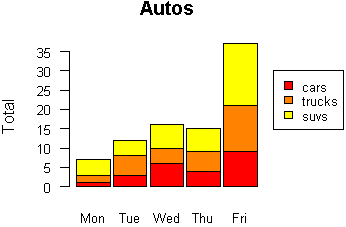
\includegraphics[width=.5\textwidth]{babs/images/bar_script4.png}
  \caption{Pengaruh nilai K terhadap akurasi}
  \label{fig:pengaruh2}
\end{figure}


\section{Subbab Tiga Satu}
Dari penjelasan di atas dapat dikatakan bahwa metodologi penelitian memiliki cakupan lebih luas daripada metode. Metode sendiri dapat diartikan sebagai cara, prosedur, atau teknik untuk menjalankan sebuah proses secara logis, terurut, dan sistematik. Metode/teknik dapat berupa metode/teknik untuk pengumpulan data, untuk analisis data, atau algoritme untuk pemecahan masalah penelitian. Terkadang metode dibedakan dari teknik dengan pemahaman bahwa teknik itu lebih khusus dan operasional daripada metode. Dalam panduan penulisan ini pemilihan istilah tersebut diserahkan kepada penulis dan pembimbingnya. Yang terpenting, apapun metode/teknik yang dipilih harus sesuai dengan sifat penelitian, masalah yang hendak diselesaikan, dan pertanyaan yang hendak dijawab. 

\subsection{Subbab Tiga Satu Satu}

Hal-hal yang perlu dijelaskan dalam metodologi penelitian adalah: 
\begin{enumerate}
  \item Tipe penelitian. Misalkan, nonimplementatif (deskriptif atau analitik) atau implementatif (pengembangan, perancangan, atau lainnya)
  \item Strategi dan rancangan penelitian 
  \begin{itemize}
    \item Strategi/metode secara umum. Misalnya, pembuatan artefak TI, studi kasus, survey, eksperimen, dan sebagainya. 
    \item Subjek atau partisipan penelitian. Siapa saja yang terlibat secara langsung dalam penelitian sebagai pelaku atau orang yang diambil datanya, serta bagaimana karakteristiknya yang dibutuhkan.
    \item Lokasi penelitian. Misalkan, di laboratorium atau studi lapangan di mana.
    \item Metode/teknik pengumpulan data. Misalnya, wawancara, observasi, kuisioner, studi dokumen.
    \item Metode/teknik analisis data dan pembahasan hasilnya. Misalnya, analisis kuantitatif secara statistik menggunakan uji t, analisis kualitatif terhadap teori A, B, dan sebagainya.
    \item Peralatan pendukung yang digunakan. Misalnya, spesifikasi piranti keras dan piranti lunak untuk menyusun kode sumber atau menguji sistem yang dibangun.
    \item Metode/teknik lainnya. Misalkan, jika strategi yang dipilih adalah pembangunan perangkat lunak, umumnya perlu dijelaskan model proses perangkat lunak yang digunakan. Sebagai catatan, Bab Metodologi Penelitian terfokus pada menjelaskan cara meneliti, sementara hasilnya dituliskan dalam bab-bab berikutnya. Oleh karena itu, dalam menjelaskan aktivitas dalam proses perangkat lunak, perlu dihindari dalam bab ini penjelasan daftar persyaratan/kebutuhan yang telah diidentifikasi, hasil perancangan, dan sebagainya. Contoh lainnya, untuk implementasi algoritma, perlu disebutkan dan dapat dideksripsikan secara singkat fungsi algoritme tersebut. Penjelasan yang lebih detil tentang algoritme tersebut dapat dimasukkan dalam bab lainnya, misalkan Bab Perancangan. 
  \end{itemize}
\end{enumerate}

Dalam mendetesiskan hal-hal di atas, penulis dapat menyusun subbab-subbab atau subbab-subbab beserta alur logikanya dengan pertimbangan sendiri di bawah supervisi pembimbing, berdasarkan relevansi dengan sifat penelitian dan aspek keterbacaan.

\subsection{Subbab Tiga Satu Dua}

Penomoran subbab disarankan tidak lebih dari 4 level (maksimal subbab X.X.X.X), tetapi sebaiknya hanya sampai 3 level. Kepala bab dan subbab tidak boleh mengandung widow atau orphan sehingga nampak menggantung atau terputus di bagian awal atau akhir sebuah halaman. Widow adalah sebuah paragraf dengan hanya satu baris pertama pada akhir halaman sedangkan sisanya berada pada halaman berikutnya. Orphan adalah baris terakhir dari satu paragraf yang tertulis pada awal suatu halaman sedangkan baris lainnya dari paragraf tersebut berada pada halaman sebelumnya.

\section{Subbab Tiga Dua}

Detesis dari subbab tiga dua, dan seterusnya.

